\documentclass[12pt]{beamer}
\usepackage[utf8]{inputenc}
%\usepackage[francais]{babel}
\usepackage[T1]{fontenc}
\usepackage{lmodern, marvosym, graphicx, multicol, lastpage}
\usepackage{geometry}
%\usepackage[hyperindex=true, colorlinks=true, breaklinks=true, linkcolor=blue]{hyperref}
\usepackage{fancyhdr, verbatim}
%\usepackage{pgf/pgf}
%\usepackage{pgf-pie-0.2.1/pgf-pie}

%\geometry{hmargin=1.5cm, vmargin=2cm}
%\addtolength{\parskip}{8pt}



\defbeamertemplate*{footline}{infolines theme}{
	\leavevmode%
		\hbox{%
				\begin{beamercolorbox}[wd=.43\paperwidth,ht=2.25ex,dp=1ex,center]{title in head/foot}%
				\usebeamerfont{title in head/foot}\insertshorttitle
				\end{beamercolorbox}%
				\begin{beamercolorbox}[wd=.50\paperwidth,ht=2.25ex,dp=1ex,center]{date in head/foot}%
				\usebeamerfont{date in head/foot}\insertshortdate{}%
				\end{beamercolorbox}%
				\begin{beamercolorbox}[wd=.07\paperwidth,ht=2.25ex,dp=1ex,left]{page in head/foot}%
				\insertframenumber{} / \inserttotalframenumber
				\end{beamercolorbox}
		}
}
\setbeamerfont{title}{series=\bfseries,size=\huge}
\setbeamerfont{subtitle}{series=\it,size=\huge}

%\usebackgroundtemplate{\includegraphics[width=\paperwidth]{img/background.jpg}}

\renewcommand{\headrulewidth}{1pt} %thikness of the line under our names
\lhead{\textbf{\titreA{} (\titreB)}}
\rhead{\emph{Bouget / Guépin / Pinhède / Vaubourr}}
\lfoot{TELECOM Nancy - PI}
\cfoot{\thepage{} / \pageref{LastPage}}
\rfoot{2012-2013}

\title{{\Large B.H. Consulting Authentication}}
\subtitle{\normalsize Industrial project}
\author{\normalsize \textbf{Intermediate presentation}}
\institute{\vspace{0.7cm}\normalsize\emph{N. Bouget, J. Guépin, M. Pinhède, J. Vaubourg}}
\date{December 13, 2012}
\titlegraphic{\vspace{1.1cm}
\includegraphics[width=60pt]{img/BHConsulting.jpg}\hfill
\includegraphics[width=80pt]{img/ul.png}\hfill
\includegraphics[width=70pt]{img/telecom-nancy.jpg}}

\begin{document}
\thispagestyle{empty}
\begin{frame}
\titlepage
\end{frame}

\title{B.H. Consulting Authentication}

%\begin{frame}{Introduction}
%    \begin{itemize}[<+->]
%	\item \emph{TELECOM Nancy} \textbf{third year} biggest project
%	\vfill
%	\item \textbf{Multiple supervisors}
%	\vfill
%	\item \textbf{Intermediate} presentation
%	\vfill
%	\item Overview of the \textbf{situation and progression}
%    \end{itemize}
%\end{frame}

\begin{frame}
    \frametitle{Outline}
    \begin{enumerate}
	\item \large{Context}
	\vfill
	\item \large{Implemented solution}
	\vfill
	\item \large{Work organization}
    \end{enumerate}
\end{frame}

\part{Context}
\frame{\partpage}
\section{Context}

\begin{frame}{TELECOM Nancy}
    \begin{center}
    
\includegraphics[width=100pt]{img/telecom-nancy.jpg}
    \end{center}
    \begin{itemize}[<+->]
	\item MSc in Computer Science, a french "Grande école"
	\vfill
	\item Accredited by the Engineer Qualification Commitee (CTI)
	\vfill
	\item Formerly named \textbf{ESIAL}, changed its name in 2012\\
    \end{itemize}
\pause
\vfill
\begin{center}
\textbf{IL \hfill\pause LE \hfill\pause SIE \hfill\pause TRS}
\end{center}
\end{frame}

\begin{frame}{Industrial project}
    \begin{itemize}[<+->]
    \item \textbf{4 students} working for a company\vfill
    \item \textbf{12 hours a week} (about 250 hours per student)\vfill
    \item Use of \textbf{real project} procedures\vfill
    \item Tackles \textbf{every aspect} of a project\vfill
    \item Learn the \textbf{project management} \vfill
    \end{itemize}
\end{frame}

\begin{frame}{B.H. Consulting}
    \begin{center}
	
\includegraphics[width=100pt]{img/BHConsulting.jpg}
    \end{center}

    \begin{itemize}[<+->]
    \item Founded by \textbf{Bertrand Pétat} in 2000\vfill
    \item \textbf{Human-scaled} company working in \textbf{network implementation}\vfill
    \item Five employees\vfill
    \end{itemize}
\end{frame}

\begin{frame}{B.H. Consulting}
\vfill
    \begin{figure}
	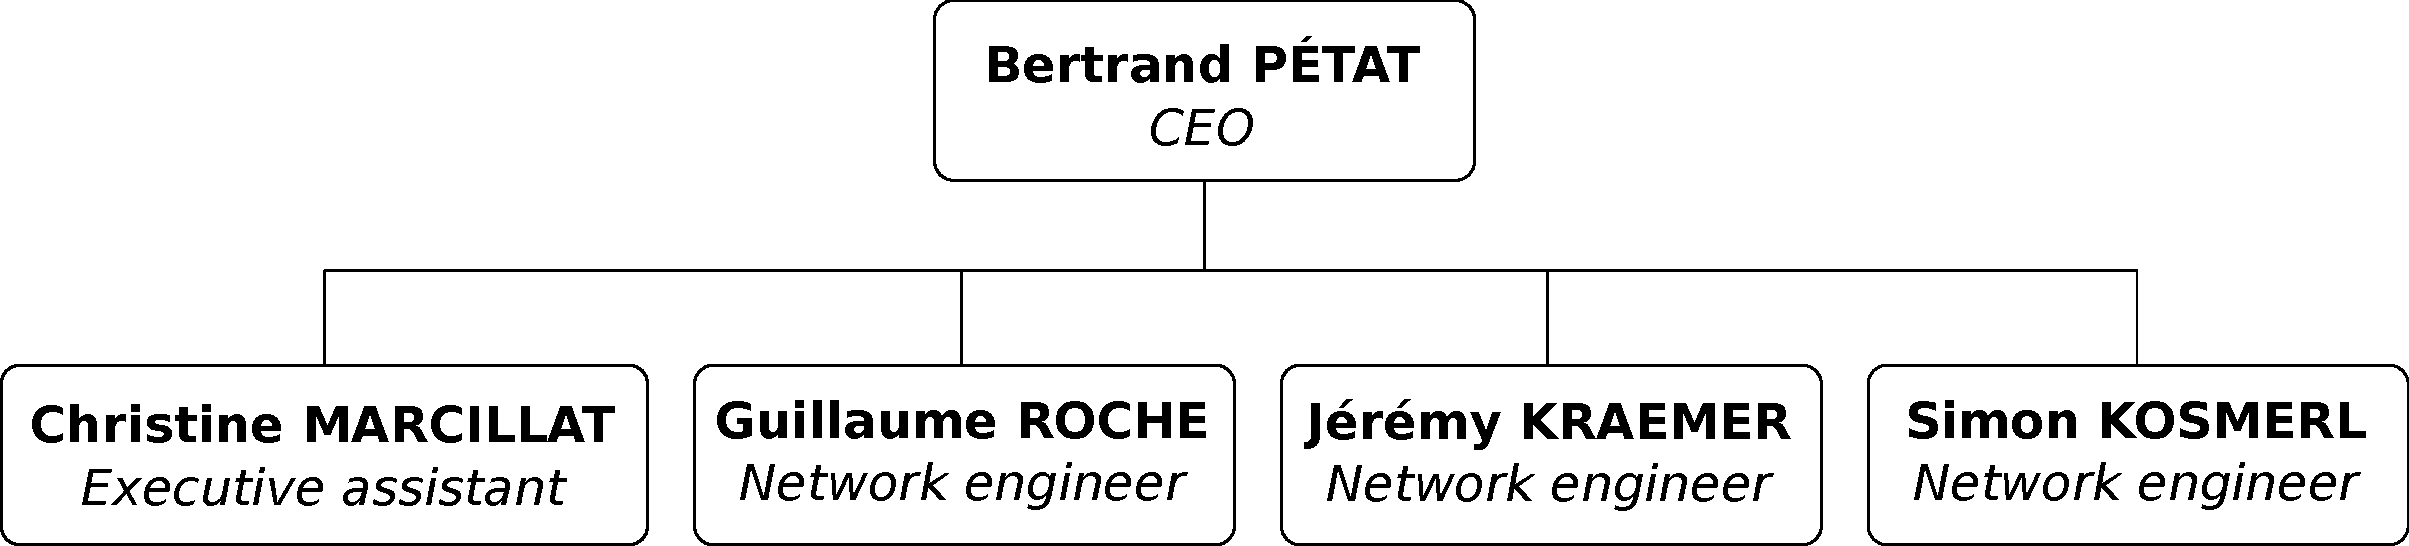
\includegraphics[width=300pt]{img/organigramme_en.pdf}
    \end{figure}
\vfill
\end{frame}

\begin{frame}{Project motivations}
    \begin{itemize}[<+->]
	\item Networks \textbf{security}
	\vfill
	\item \textbf{Access right} management
	\vfill
	\item Configurations \textbf{rollback}
	\vfill
    \end{itemize}
\pause
\textbf{--> Easy-to-install} solution

\end{frame}
    
\part{Implemented solution}
\frame{\partpage}
\section{Implemented solution}

\begin{frame}{B.H. Consulting needs}
    \begin{itemize}[<+->]
	\item \textbf{Controlled access network} for each client
	\vfill
	\item \textbf{Monitor user sessions}
	\vfill 
	\item \textbf{Offer different ways} of authentication
	\vfill
	\item \textbf{Simplify} network administration
	\vfill
	\item \textbf{Keep traces} of network configuration modifications
    \end{itemize}
\end{frame}

\begin{frame}{Implemented solution}
    \begin{center}
    \textbf{Radius server linked with MySQL and 802.1X NAS}
    \end{center}

    \pause
    \begin{itemize}[<+->]\vfill
	\item Network access controlled\vfill
	\item User accounting\vfill
	\item \textbf{Three authentication} possibilities\vfill
    \end{itemize}
    \uncover<5>{--> Installed in \textbf{one package}\vfill}
\end{frame}

\begin{frame}{802.1X}
\vfill
\begin{center}
    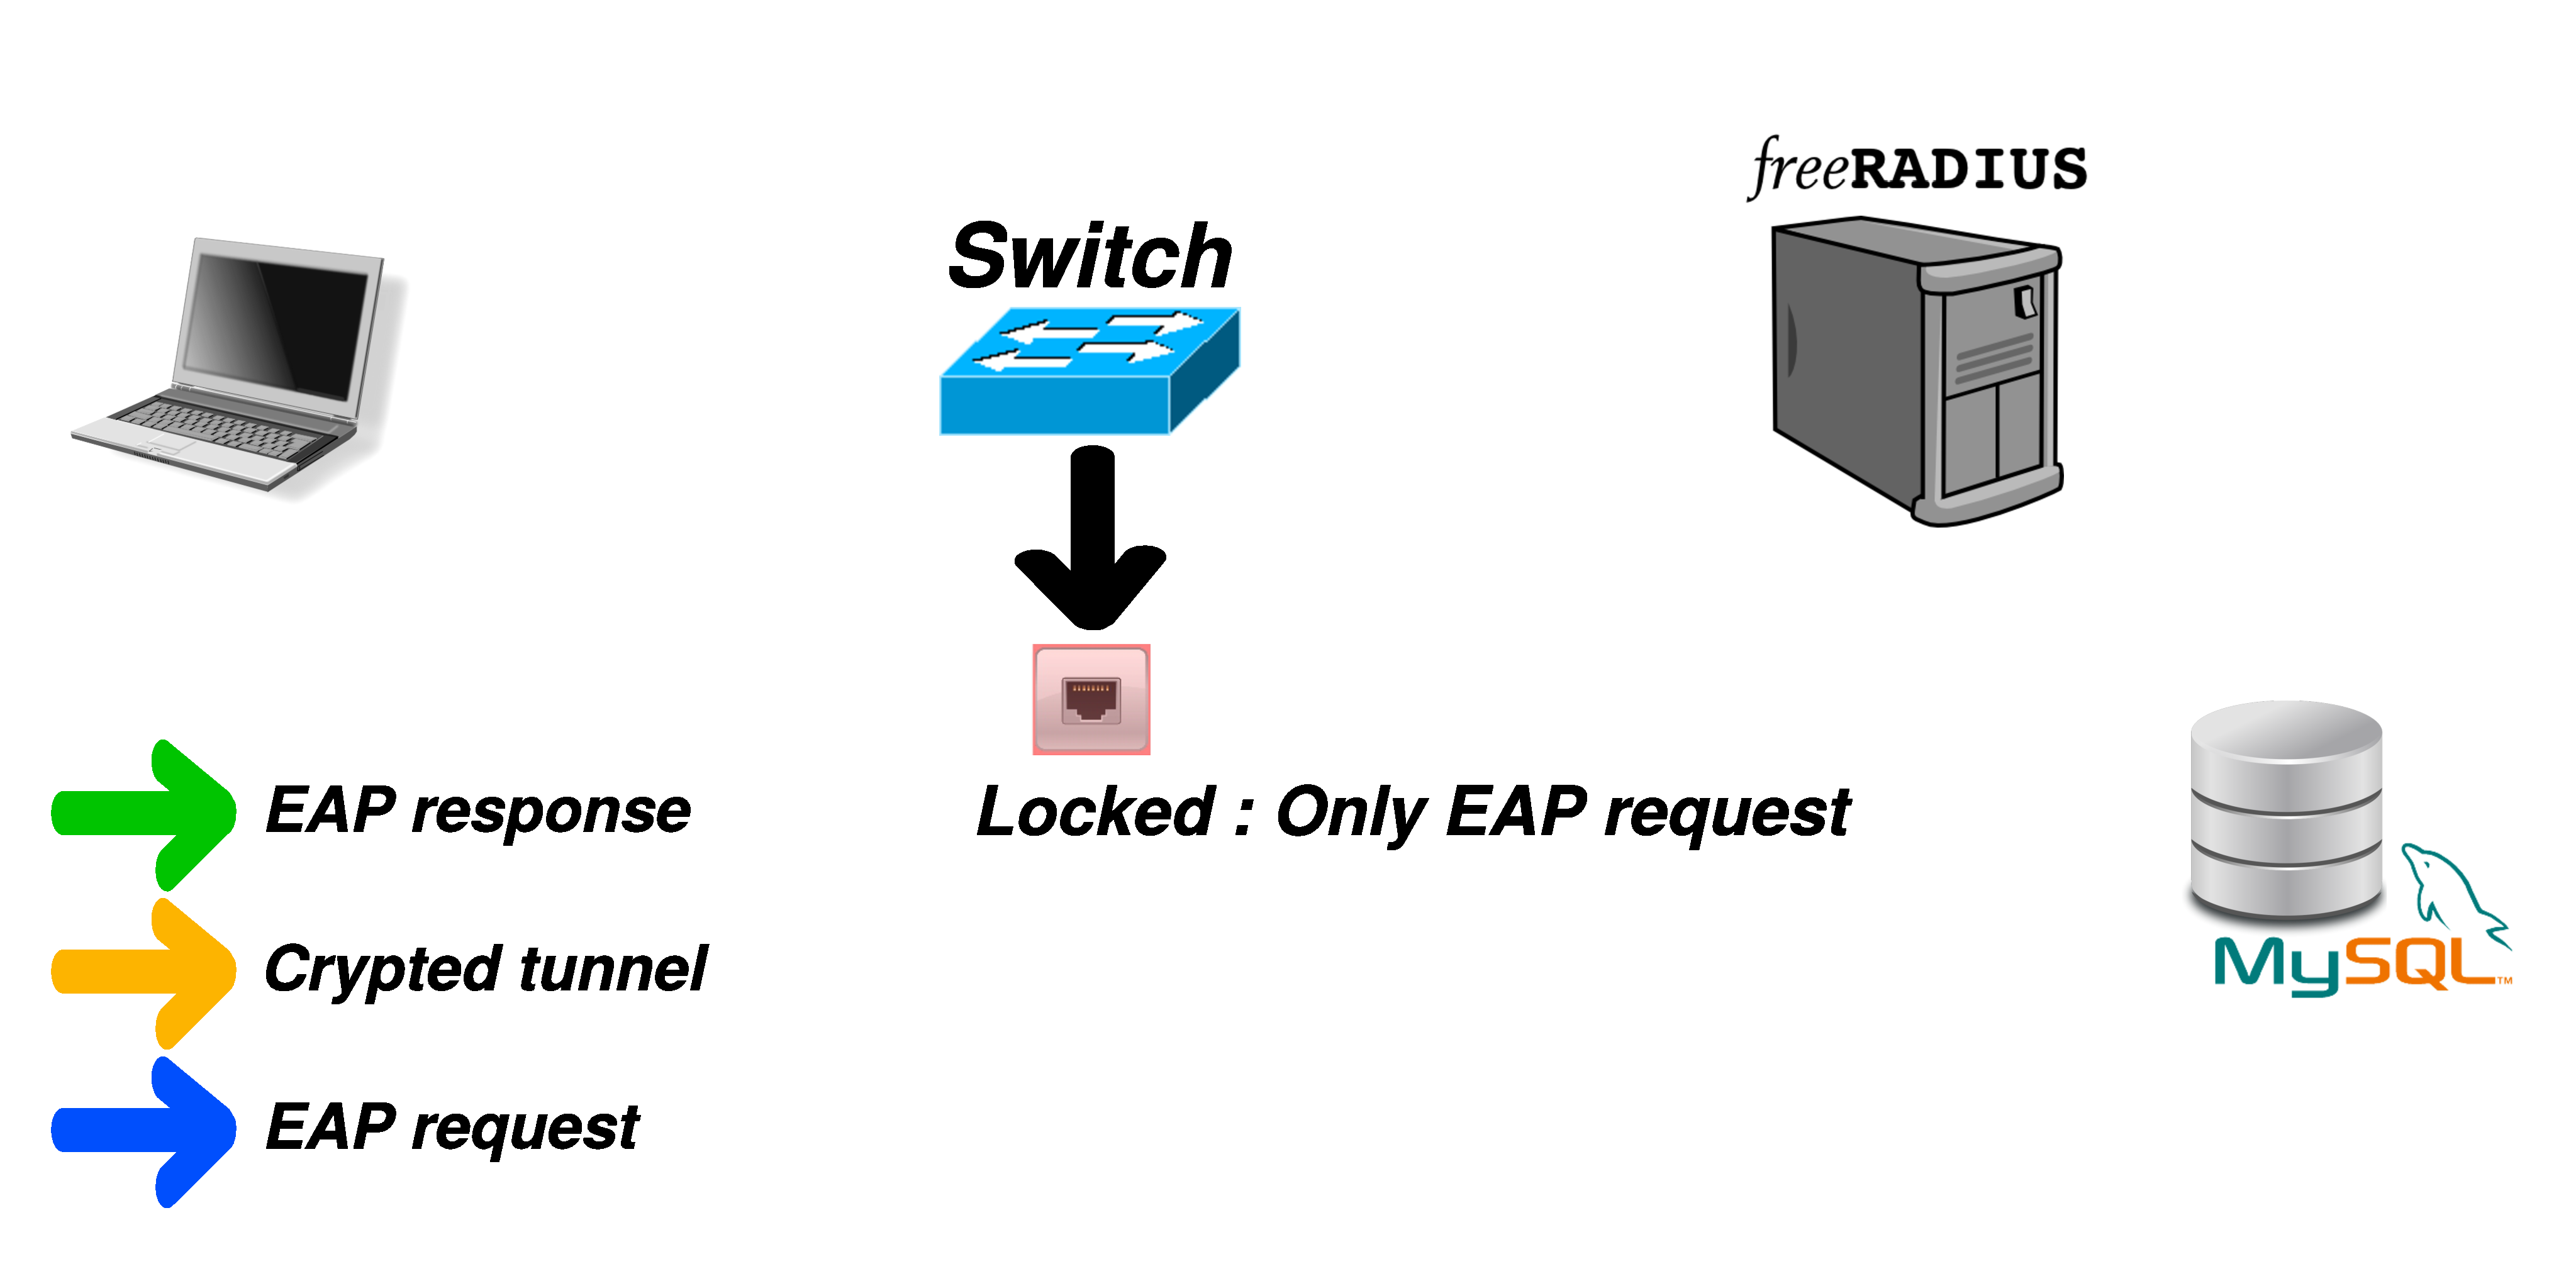
\includegraphics[width=300pt]{img/dot1x_1.pdf}
\end{center}
\vfill
\end{frame}

\begin{frame}[noframenumbering]{802.1X}
\vfill
\begin{center}
    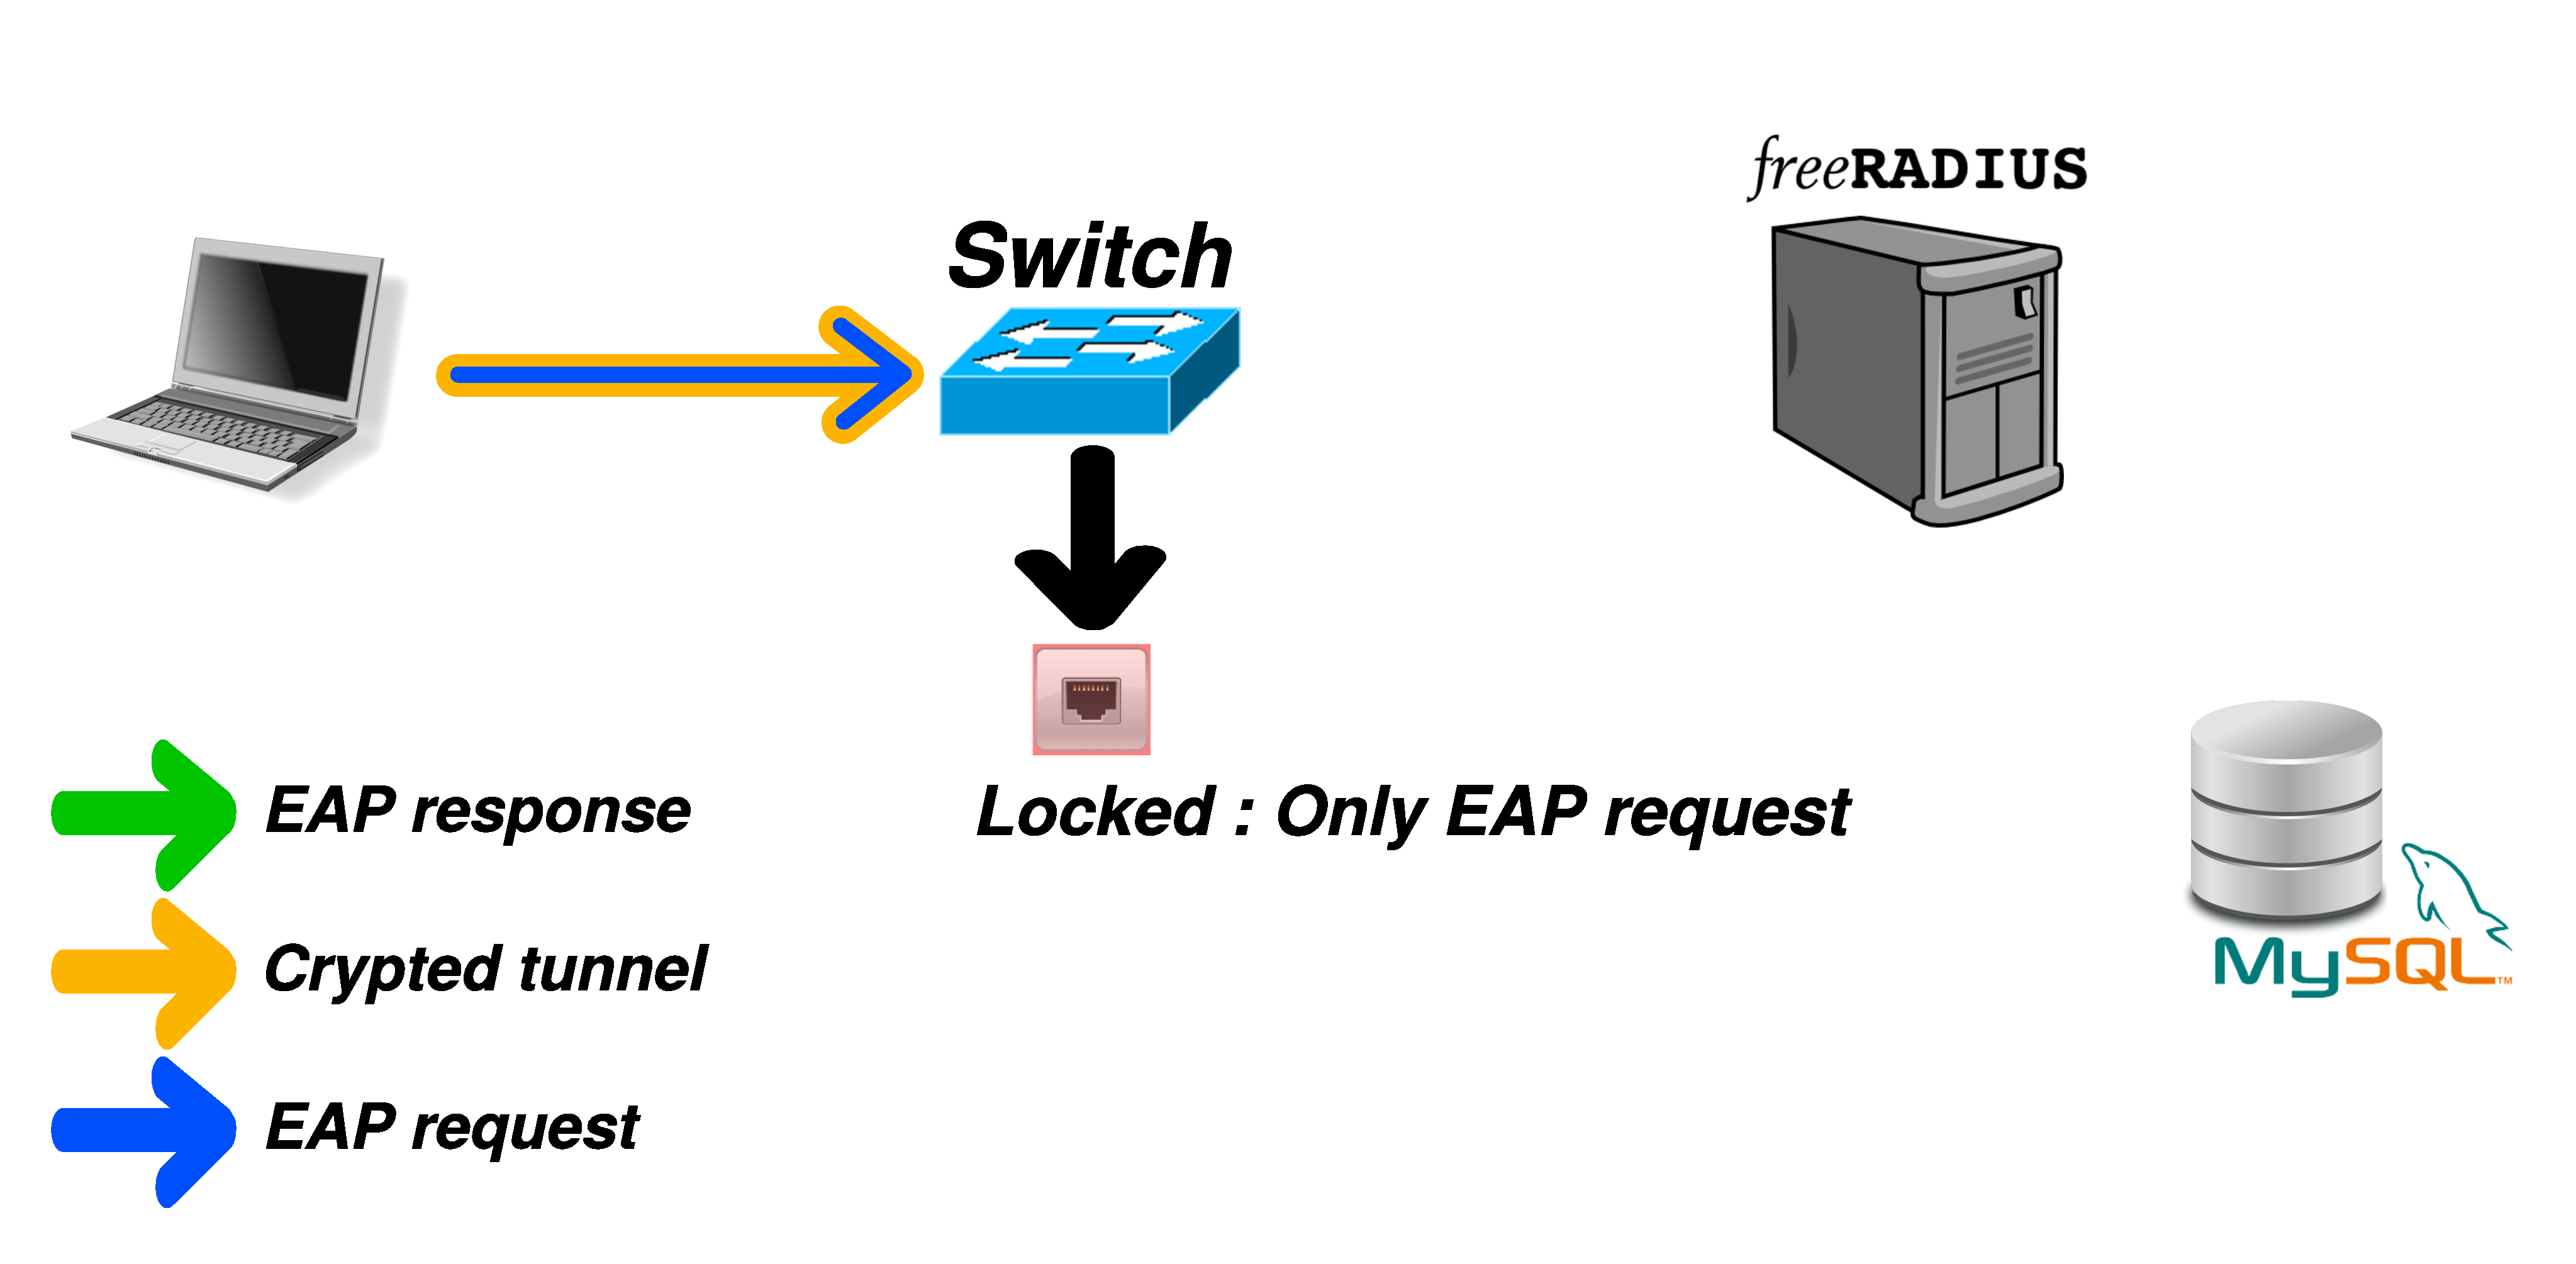
\includegraphics[width=300pt]{img/dot1x_2.pdf}
    %\addtocounter{framenumber}{-1}
\end{center}
\vfill
\end{frame}

\begin{frame}[noframenumbering]{802.1X}
\vfill
\begin{center}
    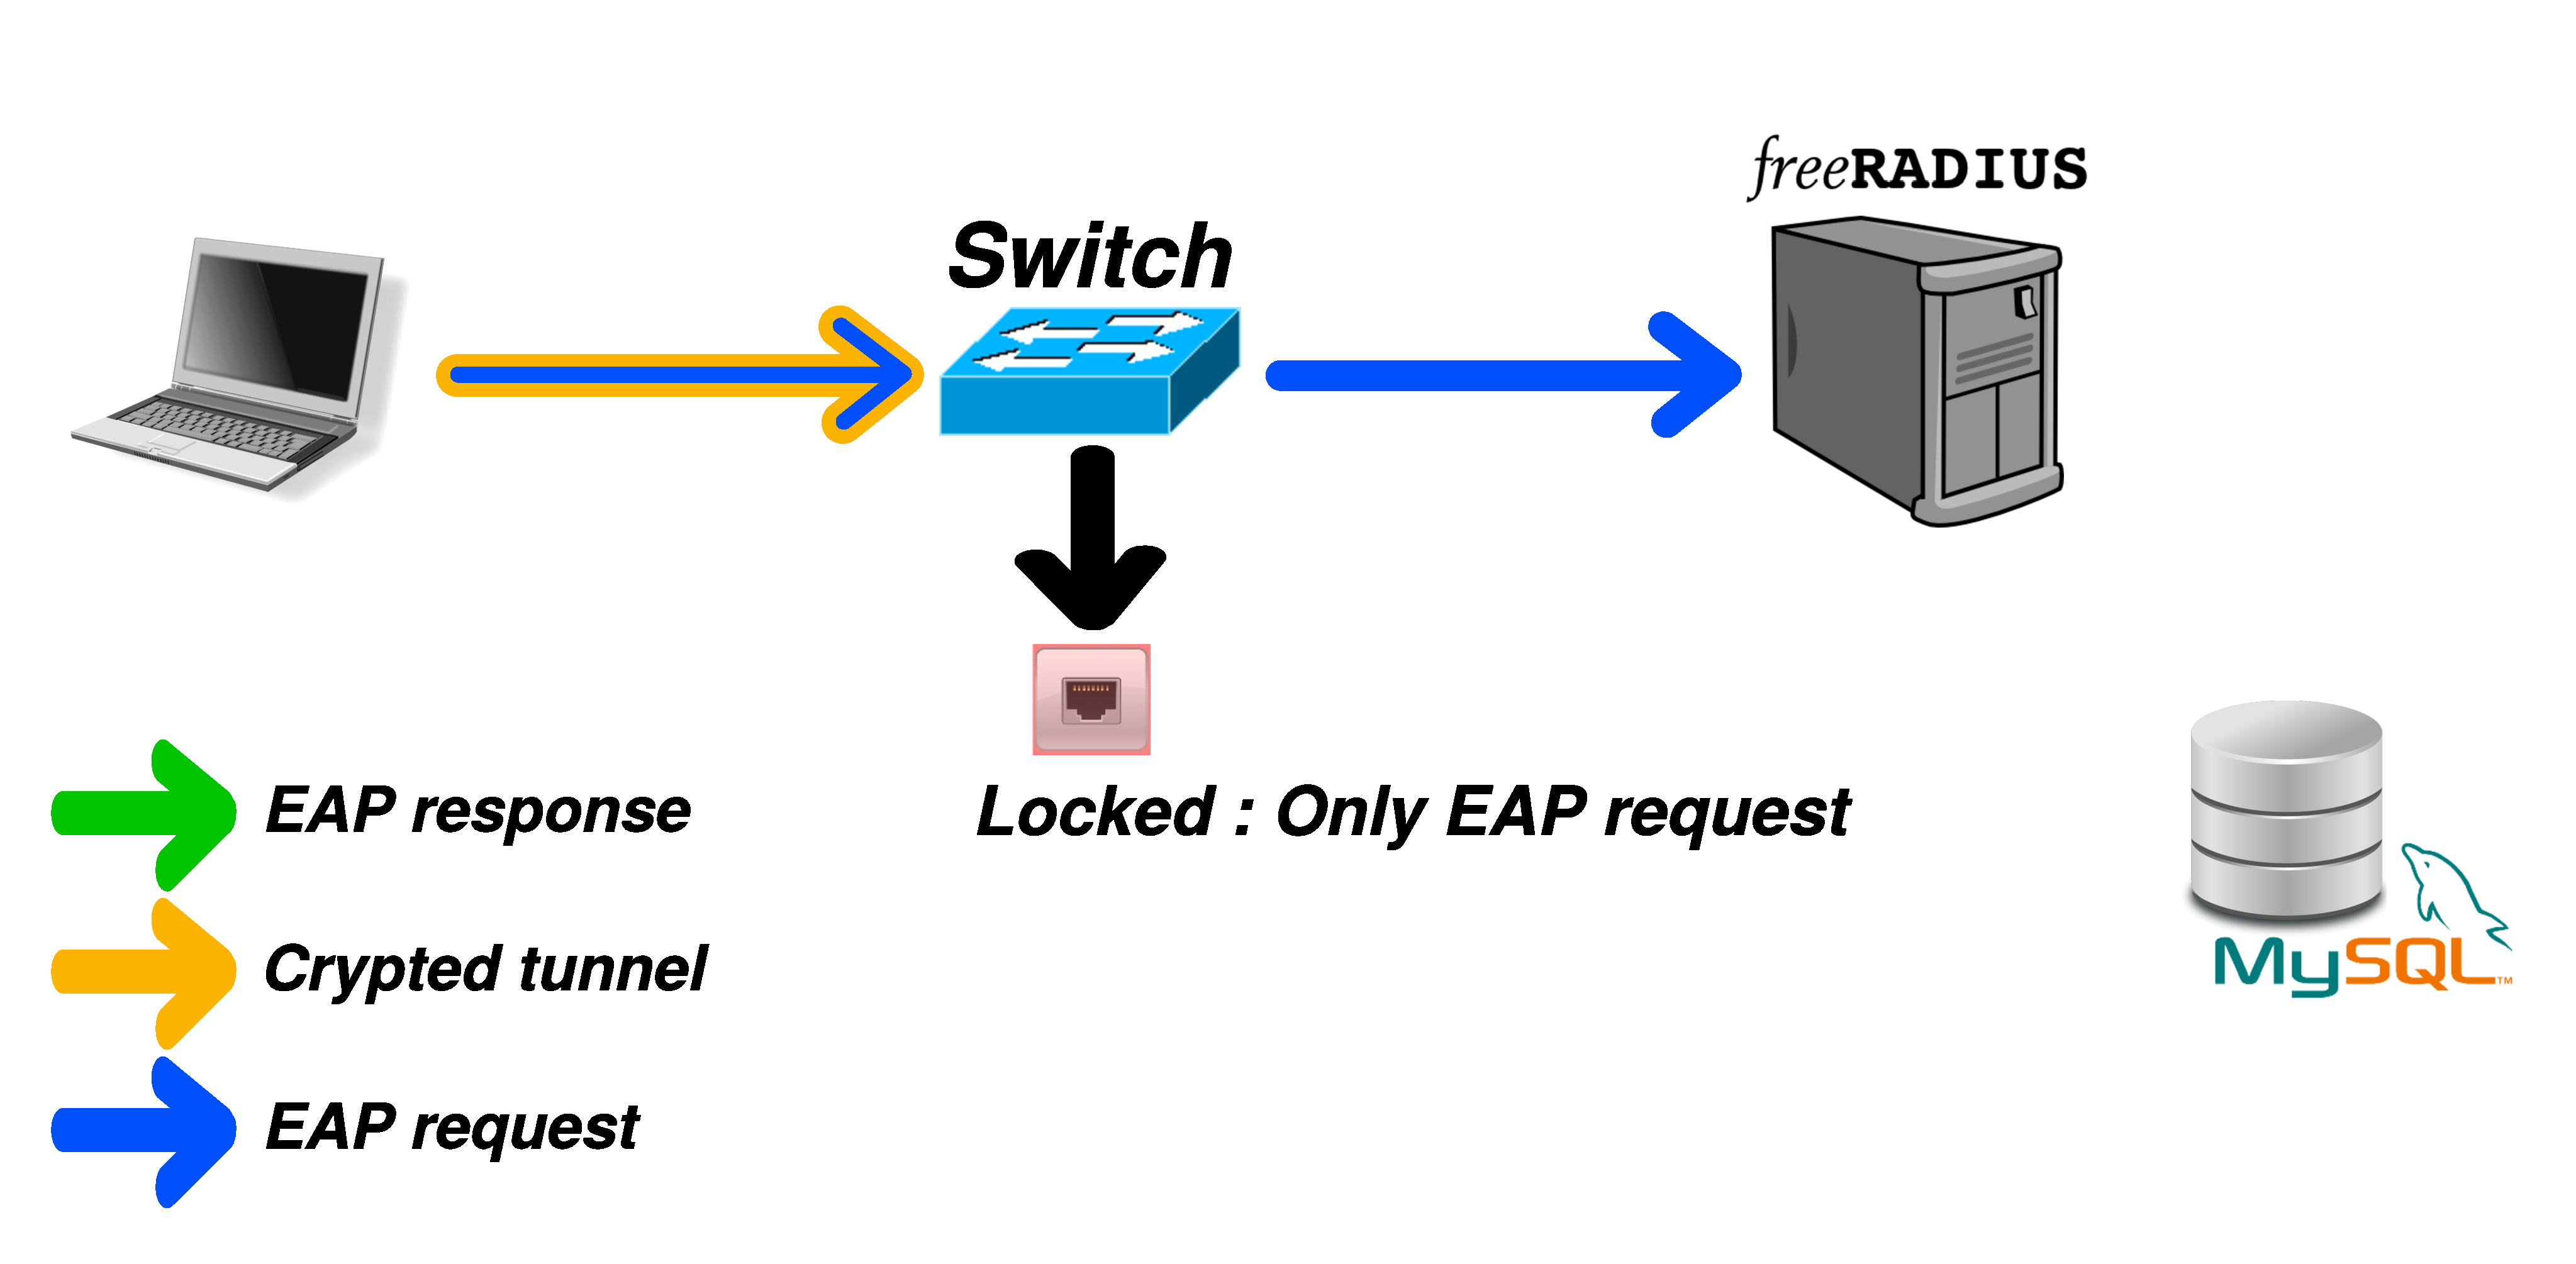
\includegraphics[width=300pt]{img/dot1x_3.pdf}
    %\addtocounter{framenumber}{-1}
\end{center}
\vfill
\end{frame}

\begin{frame}[noframenumbering]{802.1X}
\vfill
\begin{center}
    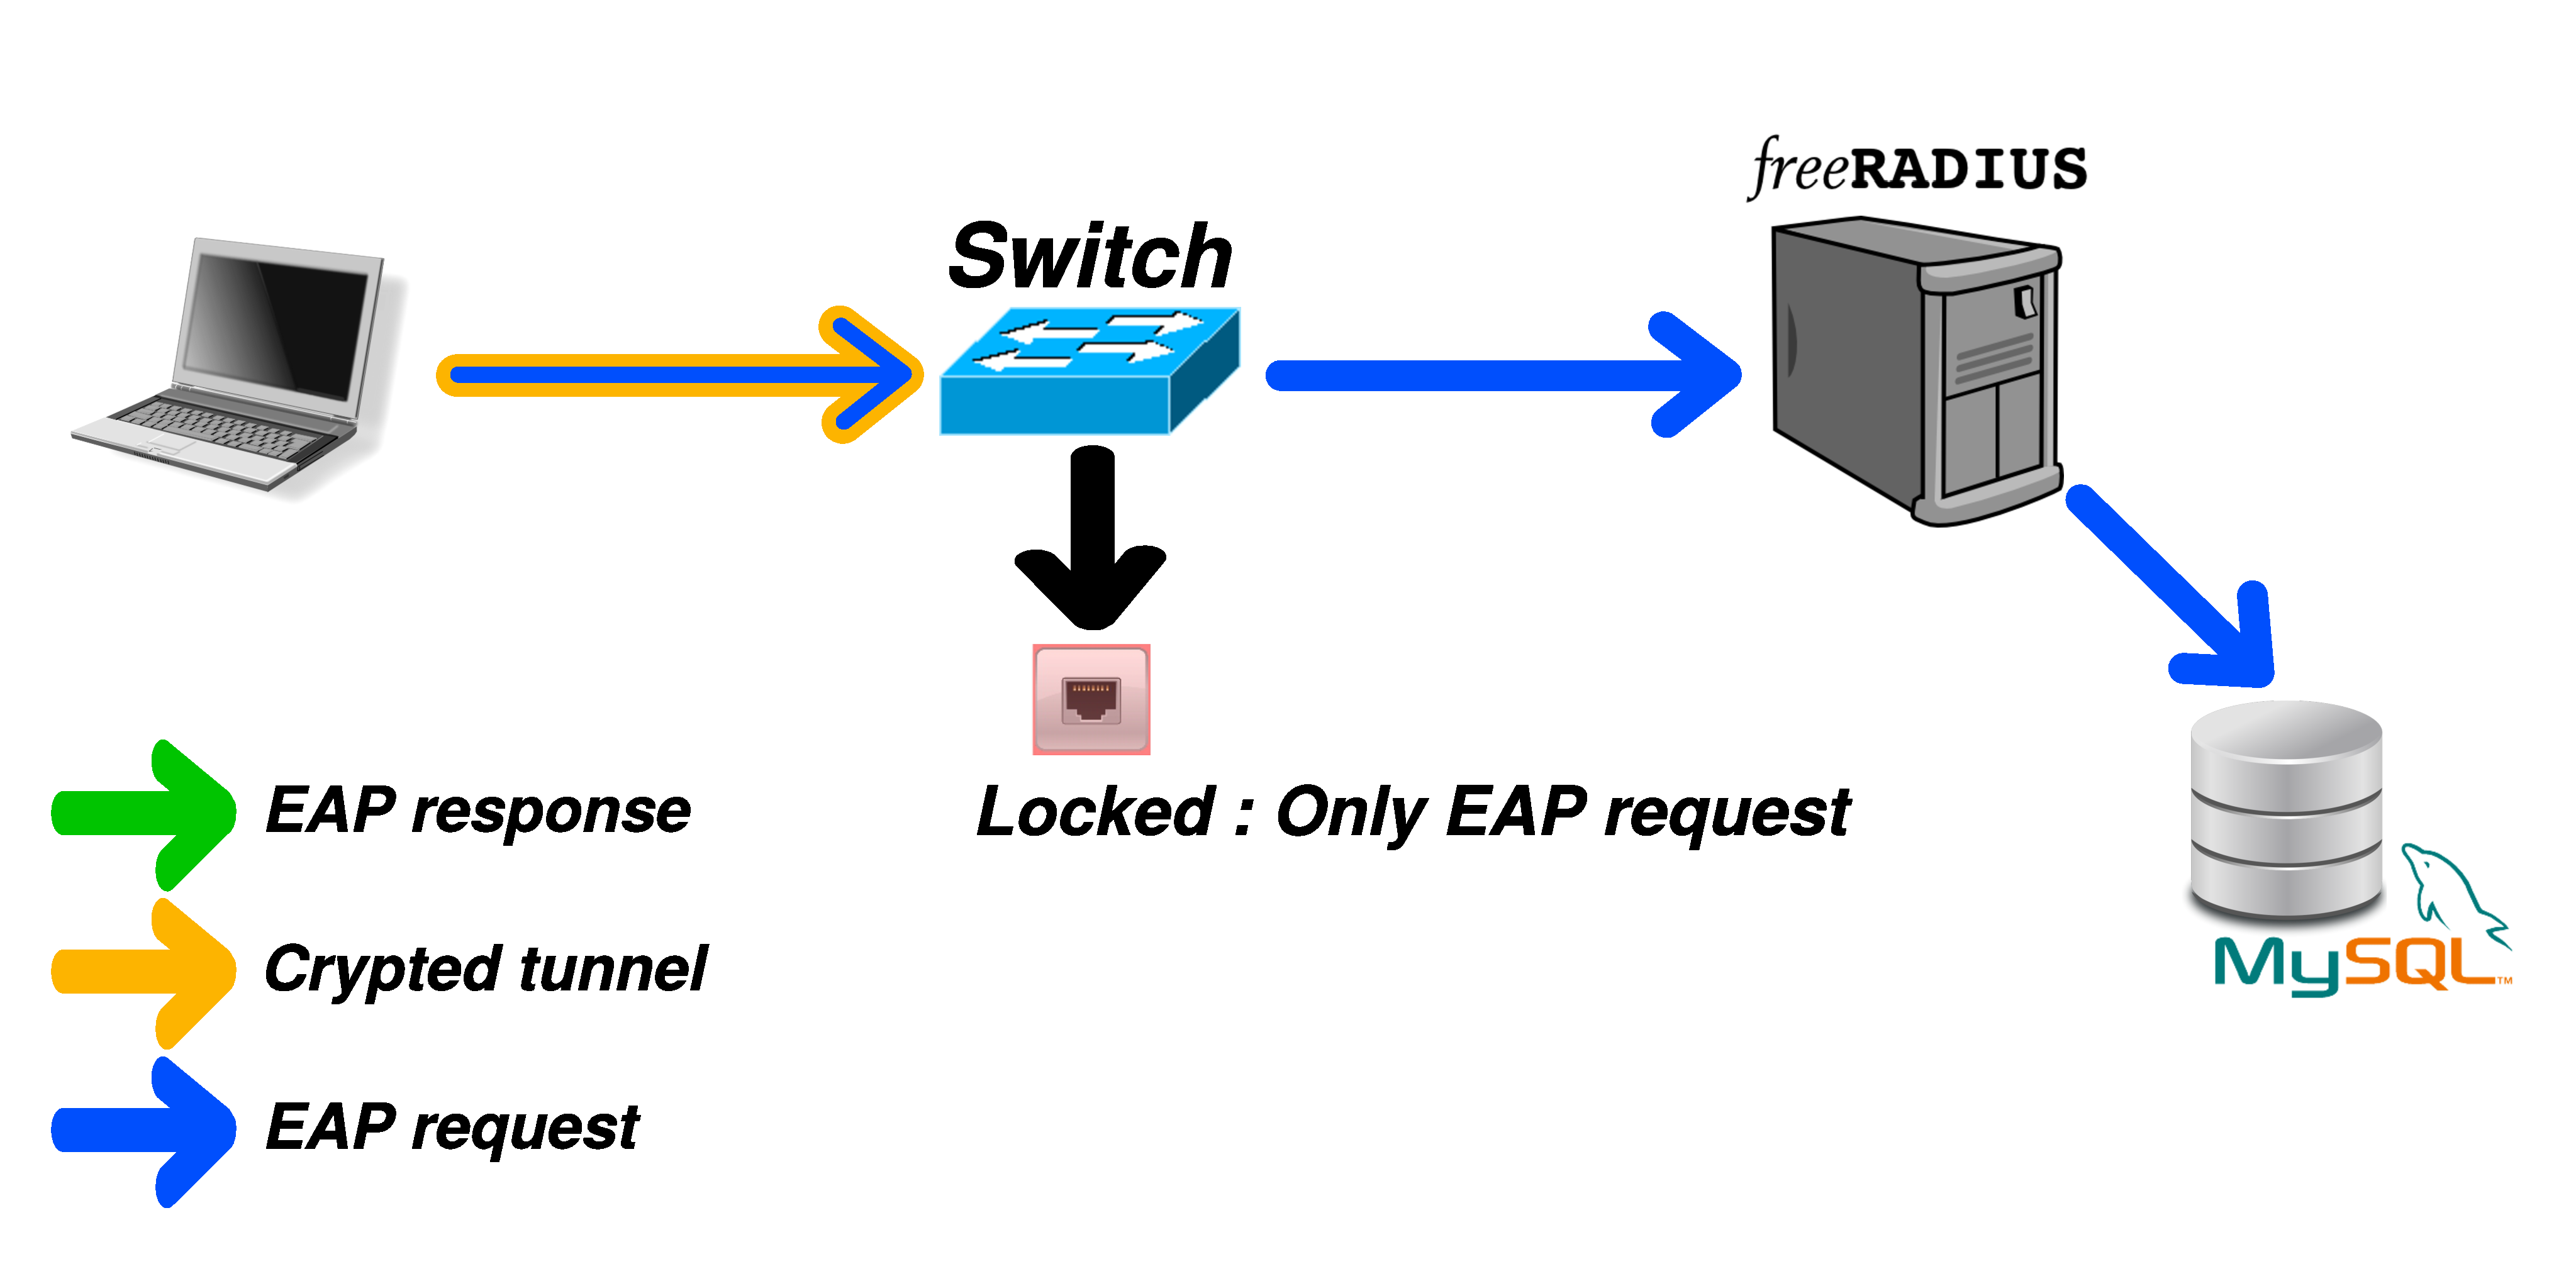
\includegraphics[width=300pt]{img/dot1x_4.pdf}
    %\addtocounter{framenumber}{-1}
\end{center}
\vfill
\end{frame}

\begin{frame}[noframenumbering]{802.1X}
\vfill
\begin{center}
    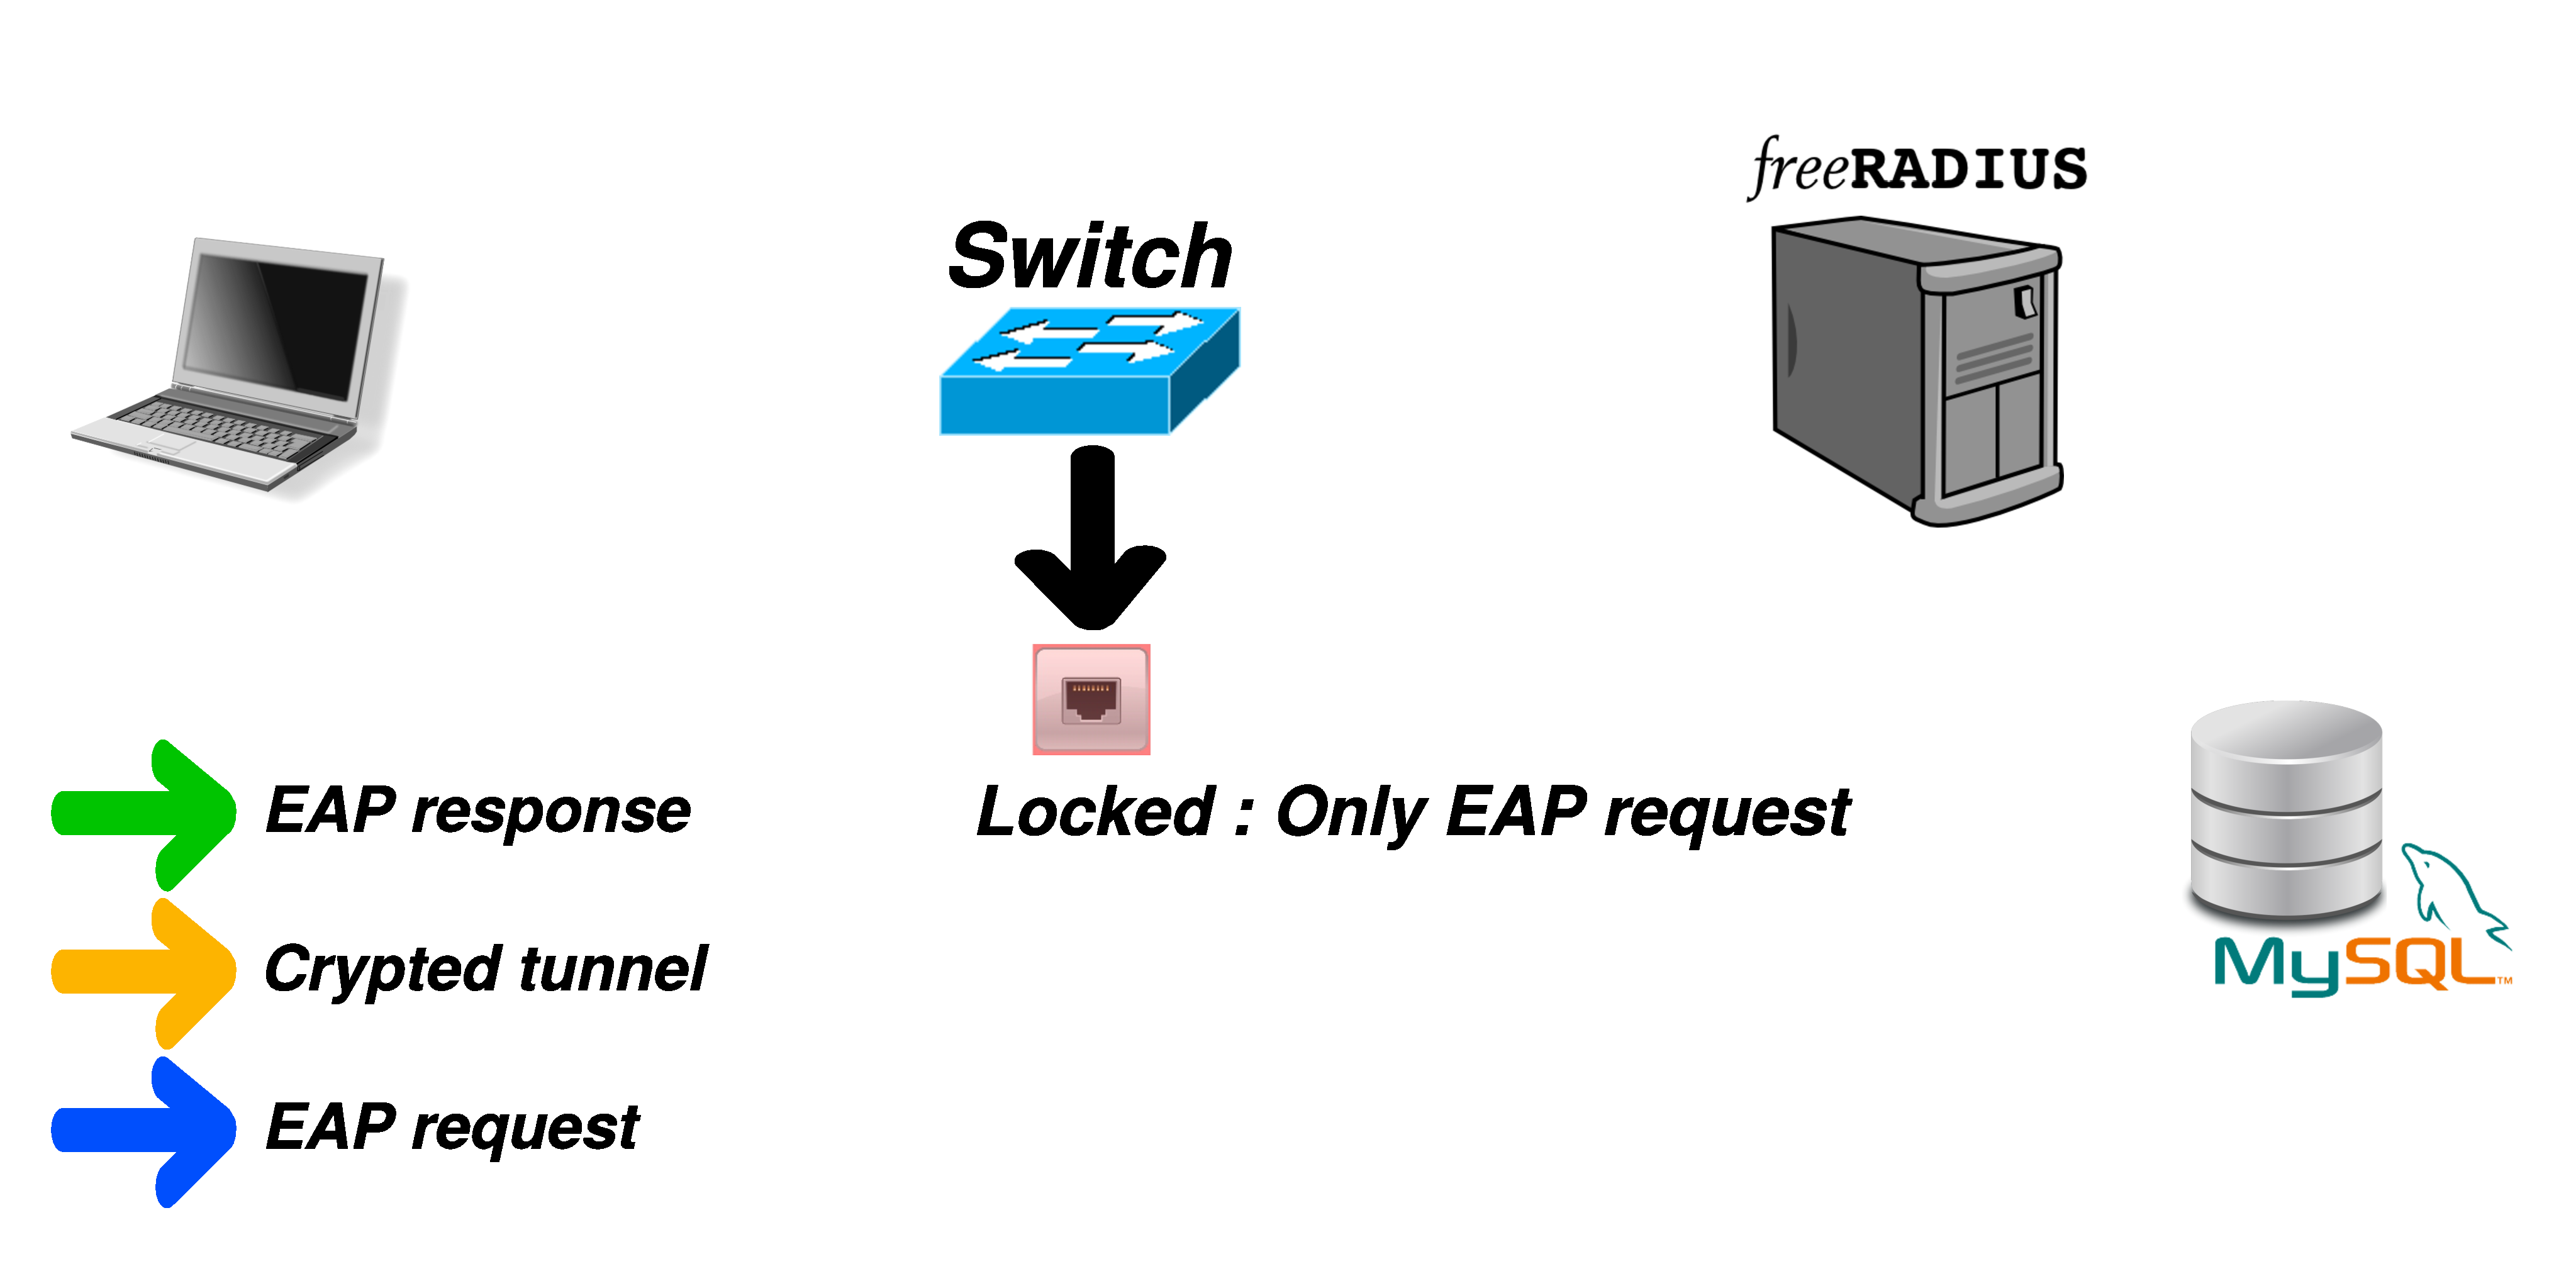
\includegraphics[width=300pt]{img/dot1x_1.pdf}
    %\addtocounter{framenumber}{-1}
\end{center}
\vfill
\end{frame}

\begin{frame}[noframenumbering]{802.1X}
\vfill
\begin{center}
    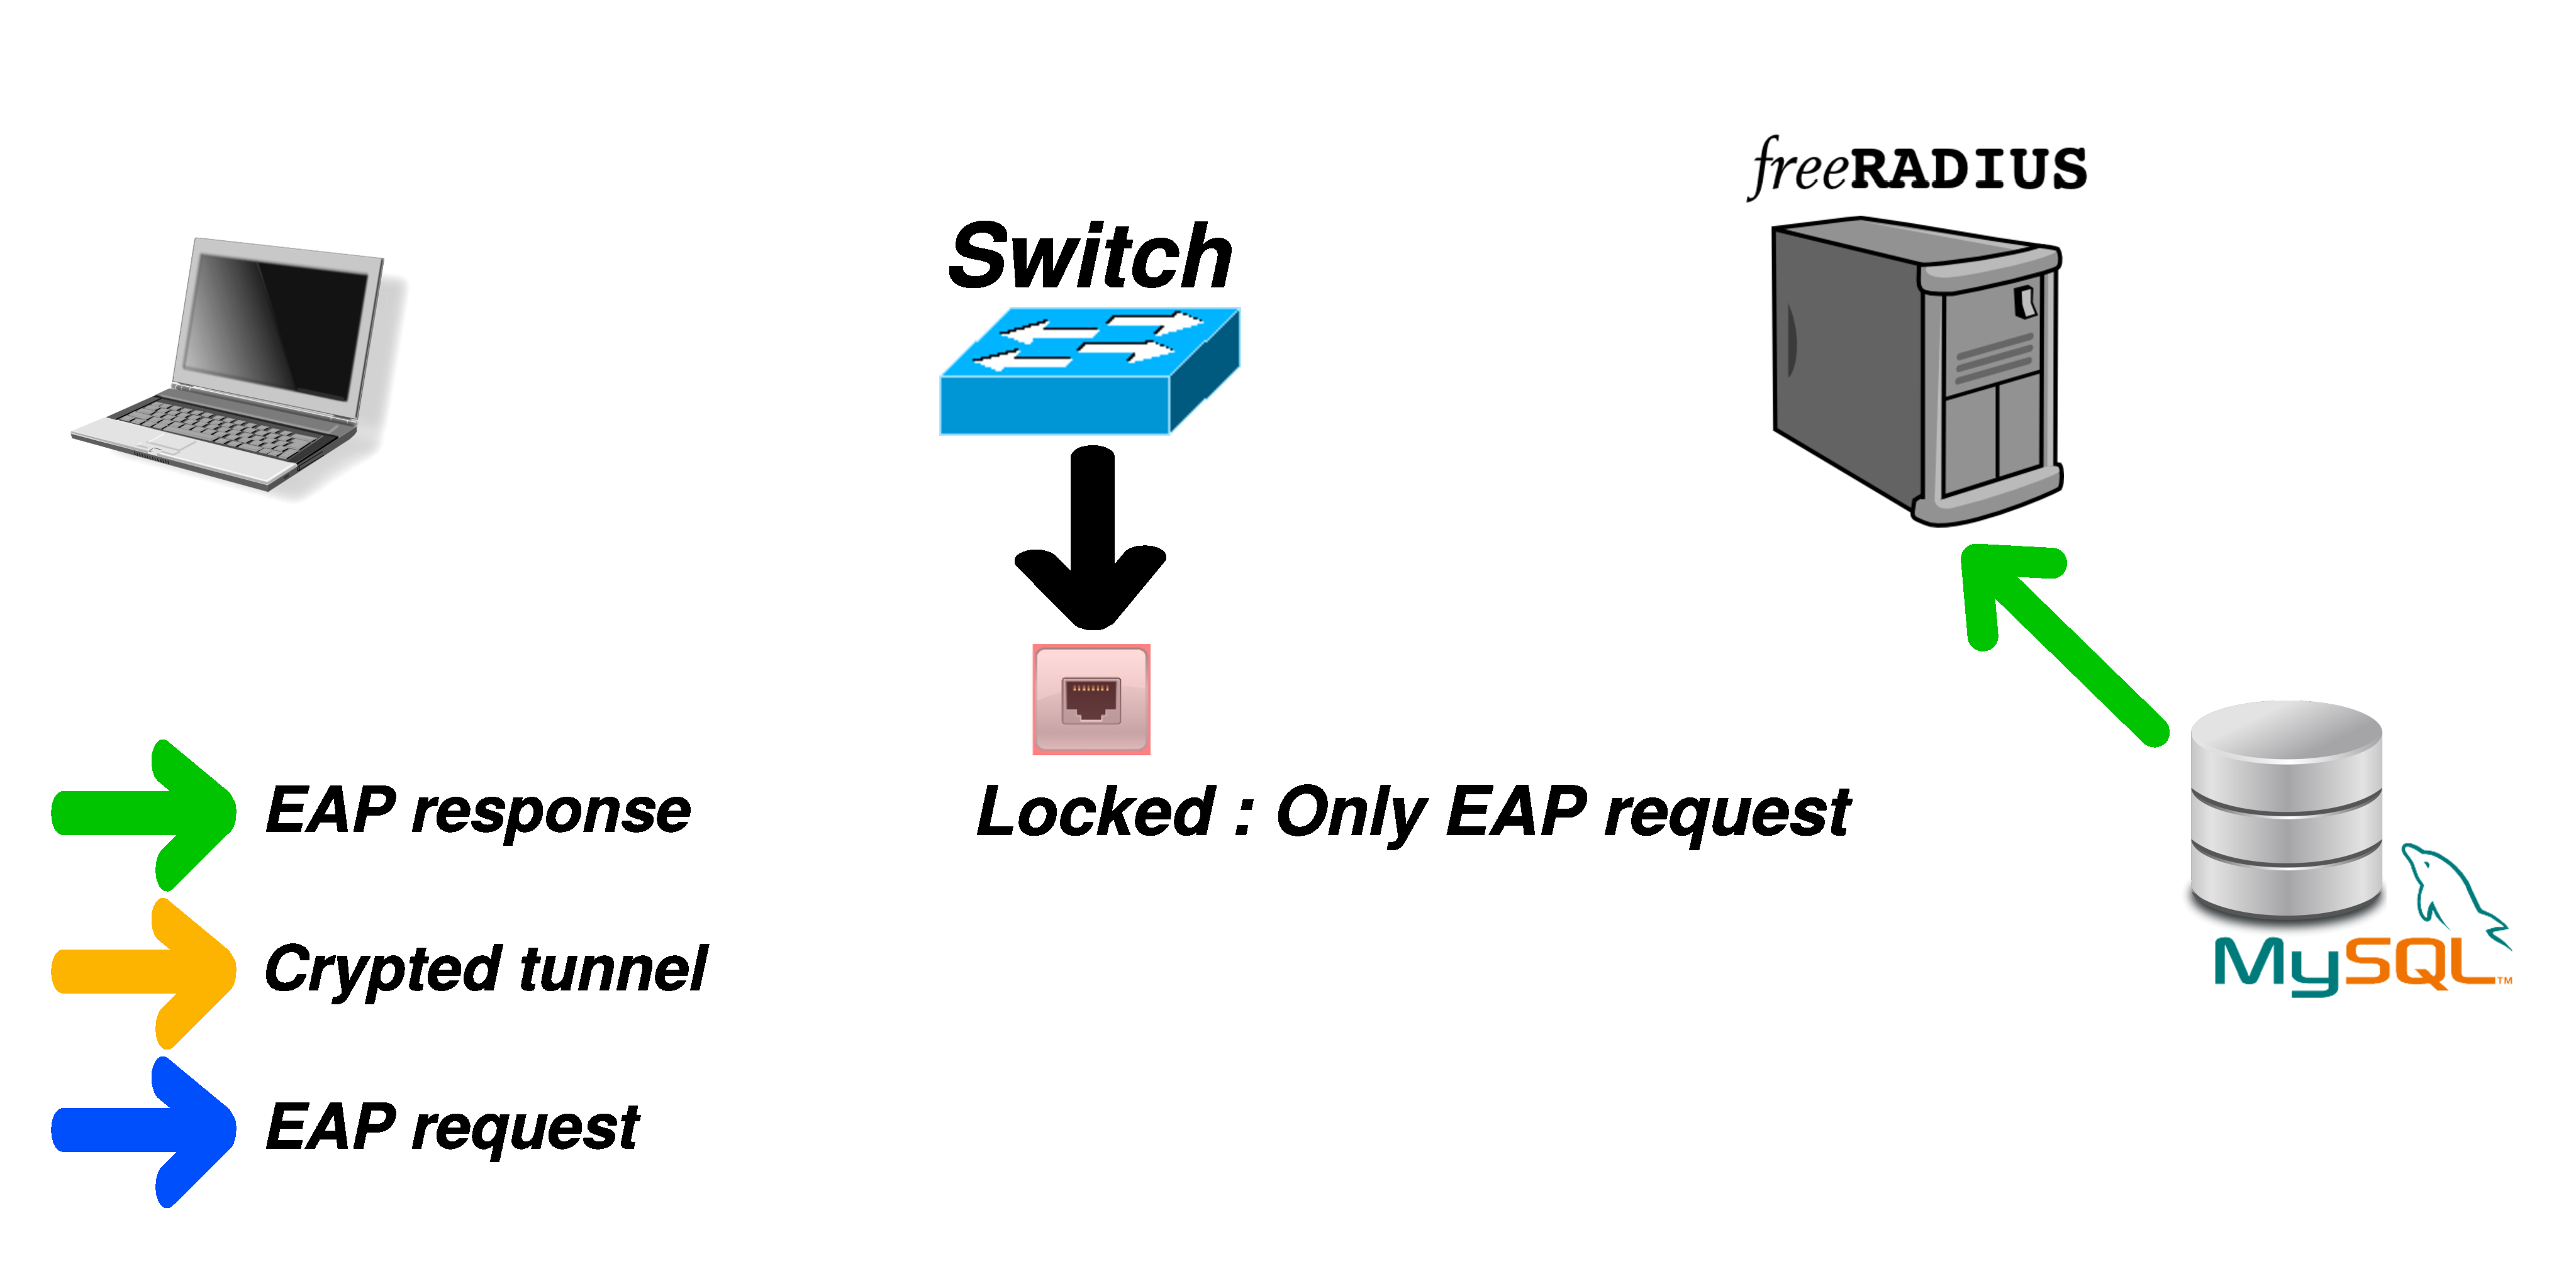
\includegraphics[width=300pt]{img/dot1x_5.pdf}
    %\addtocounter{framenumber}{-1}
\end{center}
\vfill
\end{frame}

\begin{frame}[noframenumbering]{802.1X}
\vfill
\begin{center}
    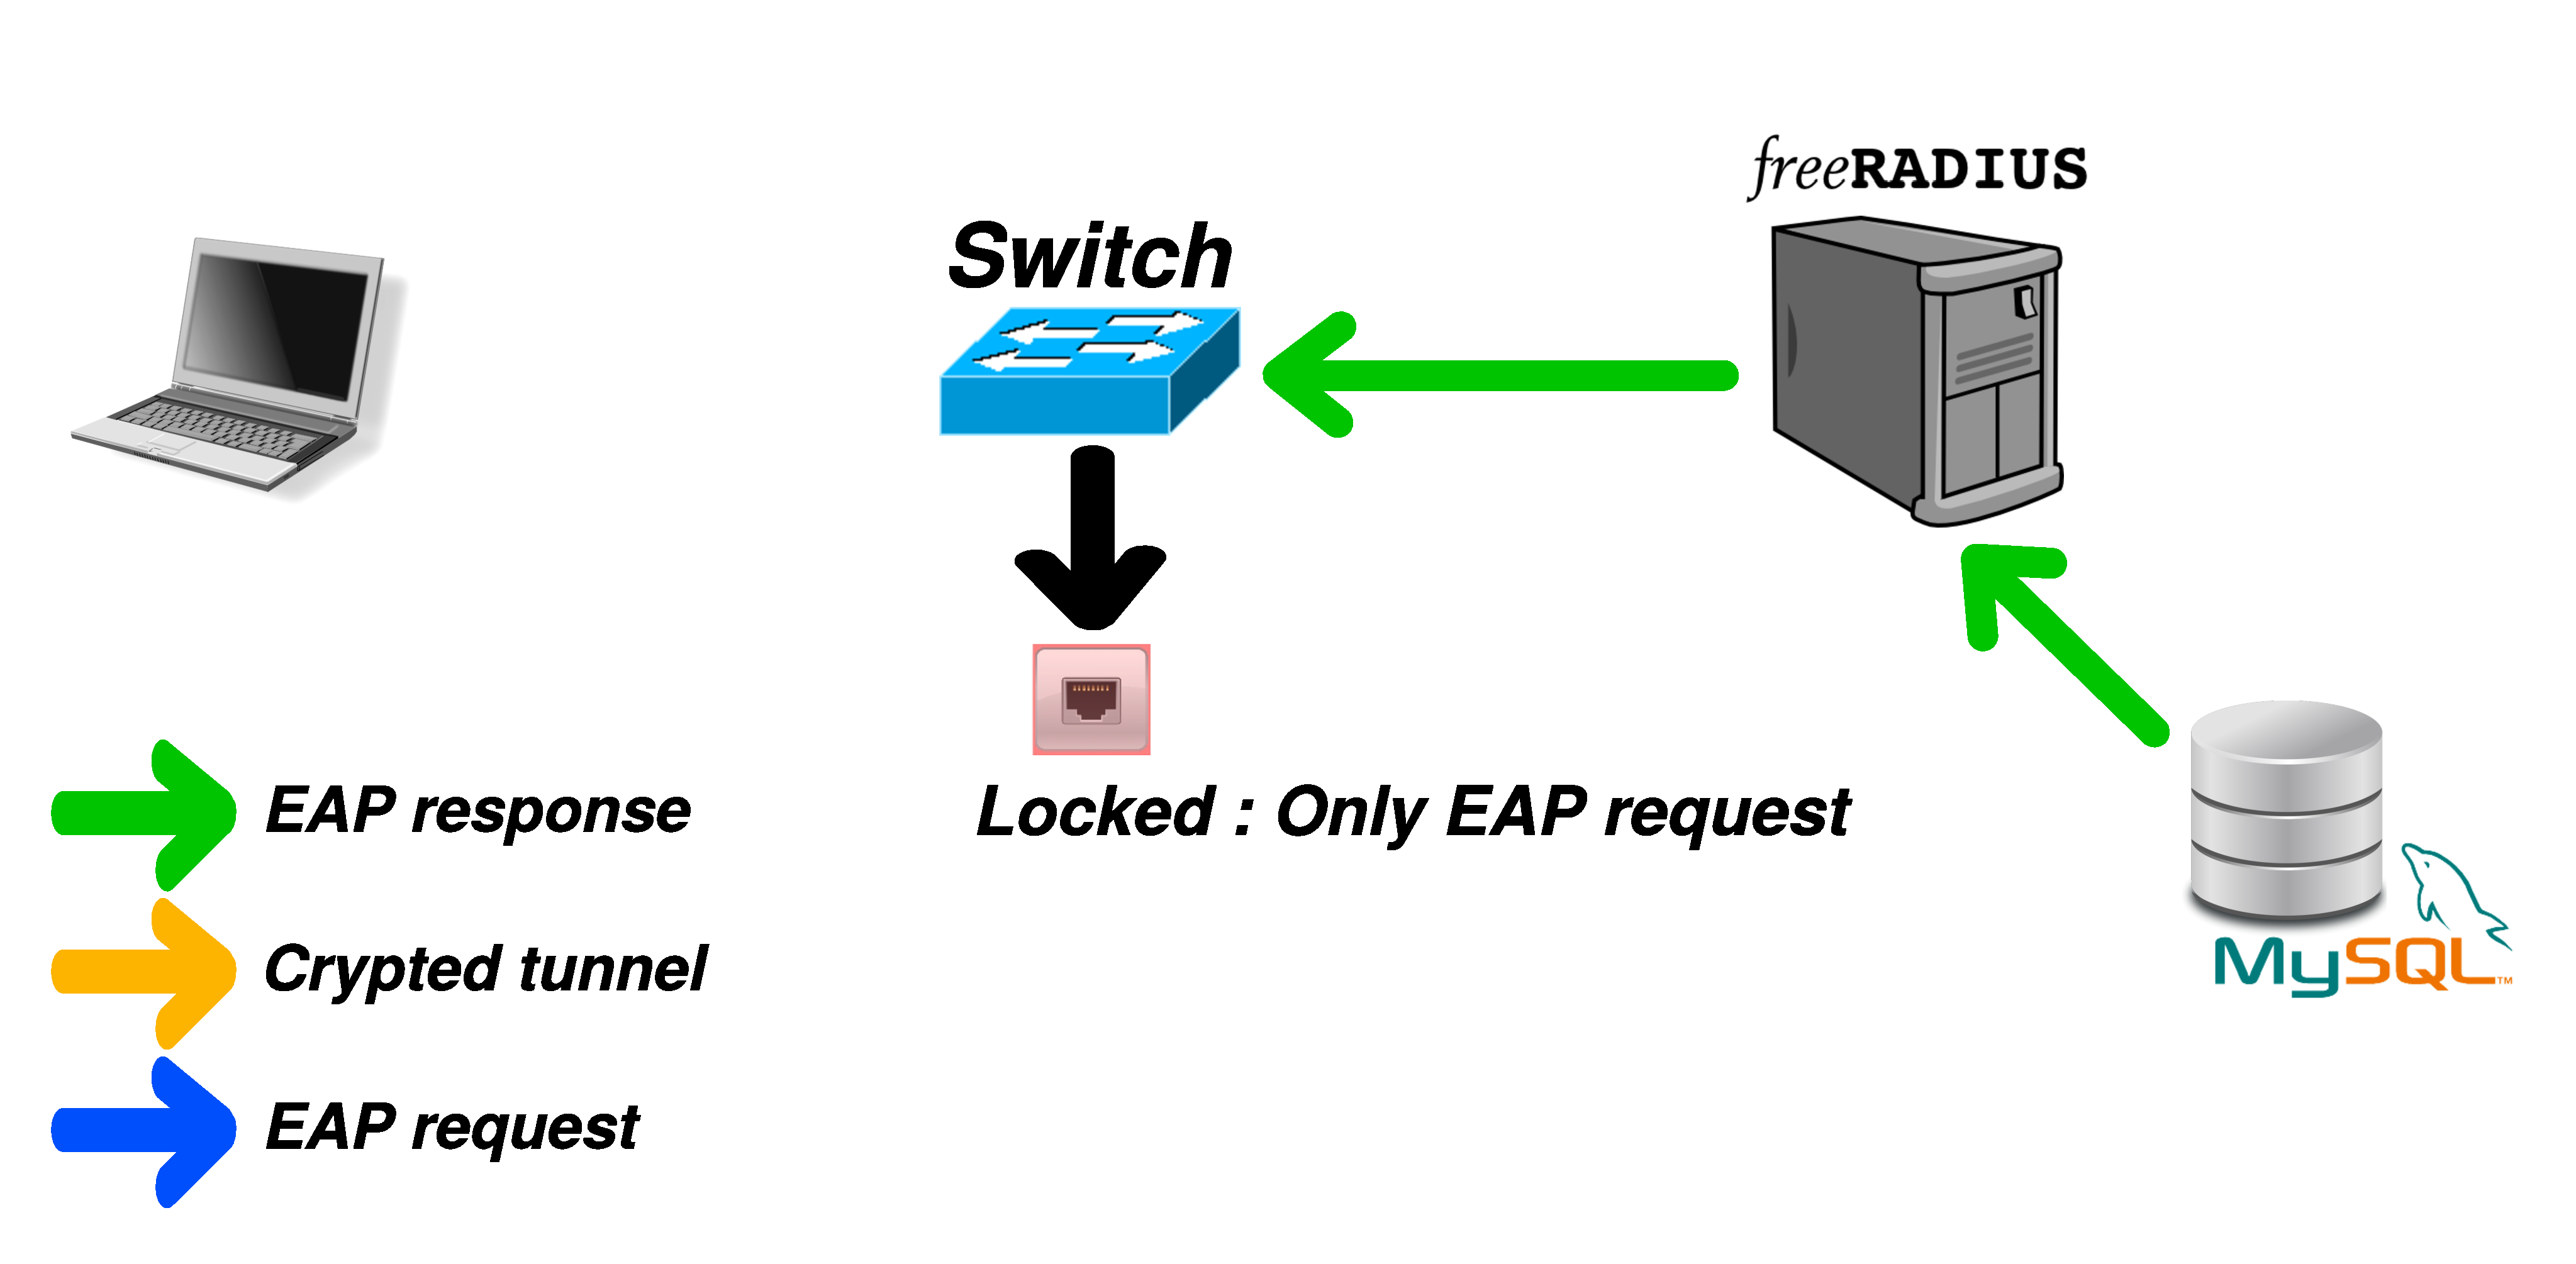
\includegraphics[width=300pt]{img/dot1x_6.pdf}
    %\addtocounter{framenumber}{-1}
\end{center}
\vfill
\end{frame}

\begin{frame}{802.1X}
\vfill
\begin{center}
    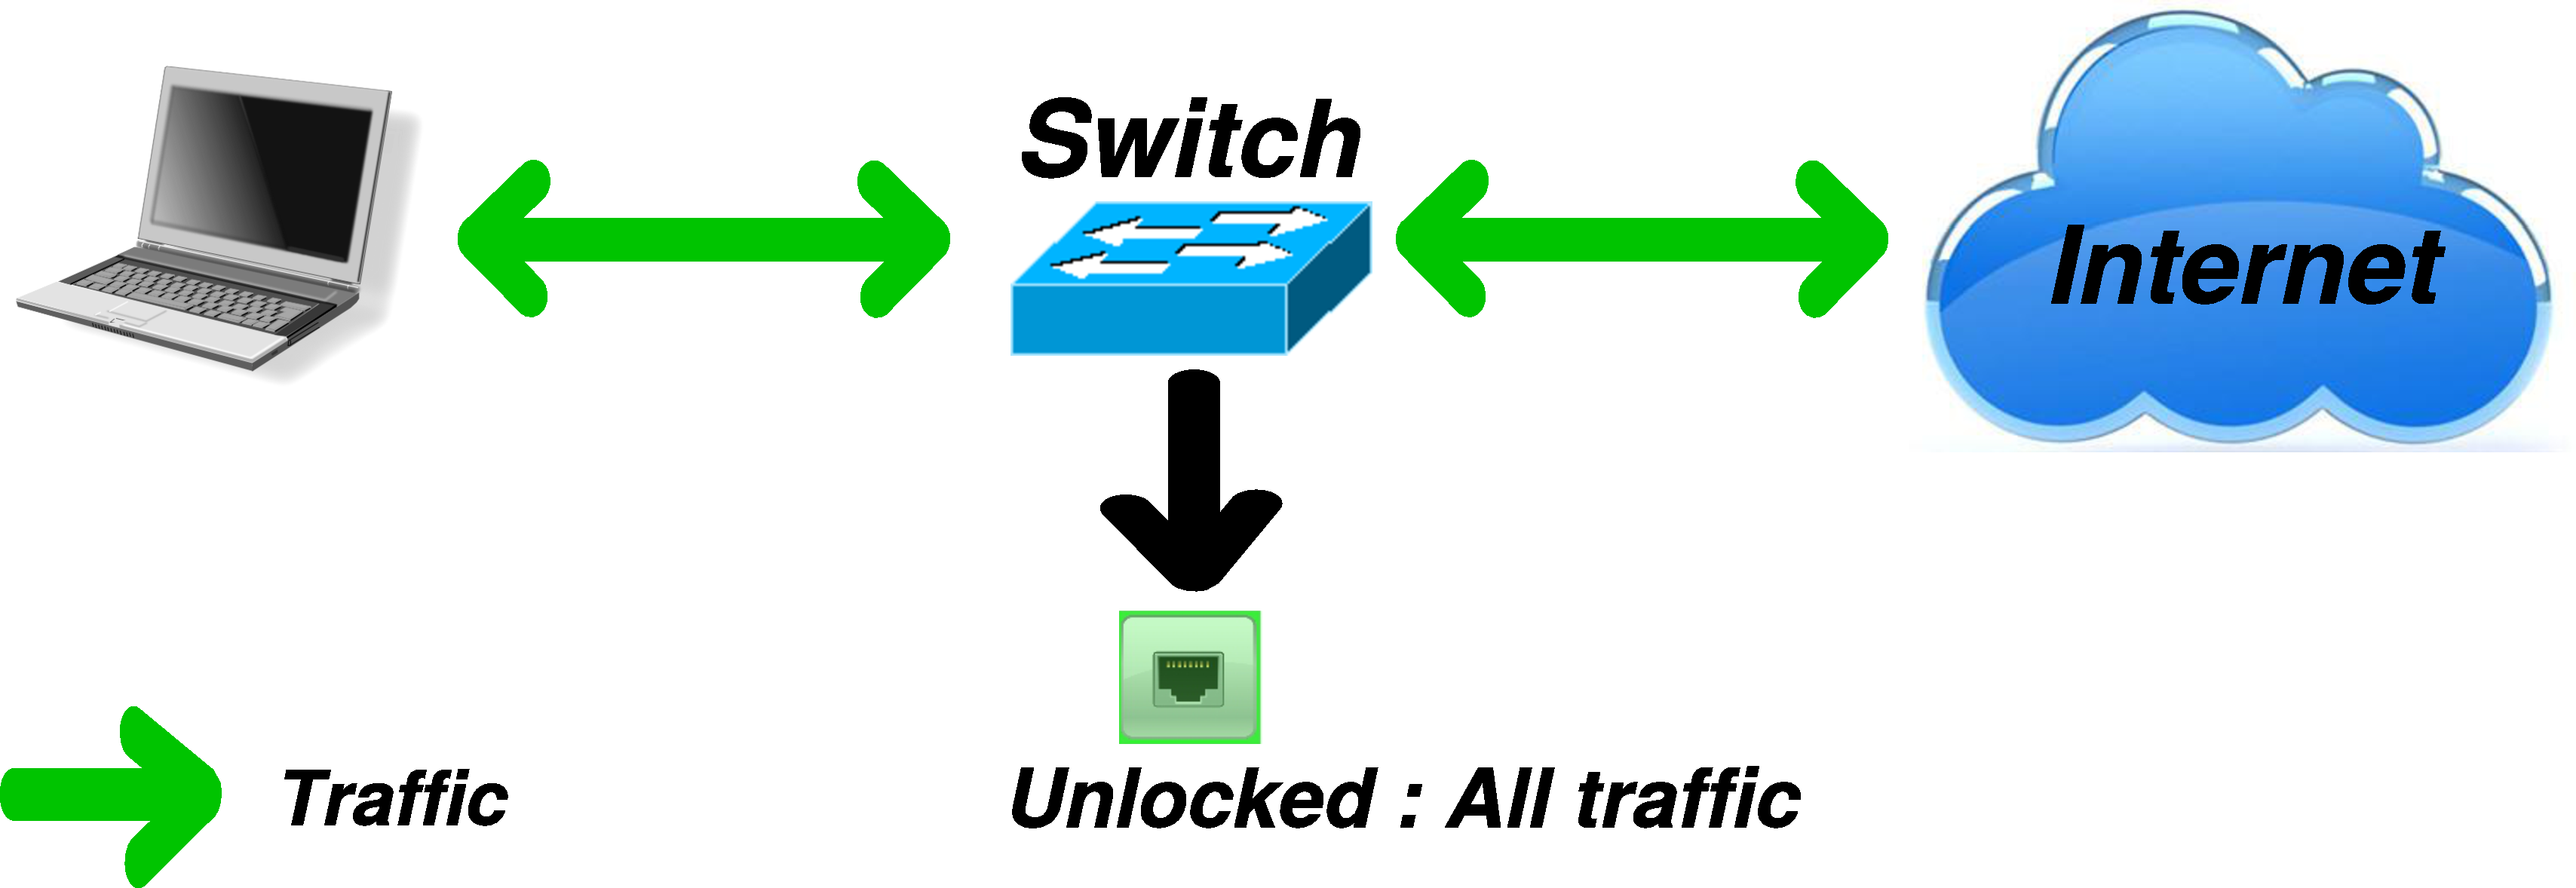
\includegraphics[width=300pt]{img/dot1x_7.pdf}
    %\addtocounter{framenumber}{-1}
\end{center}
\vfill
\end{frame}

\begin{frame}{User interface}
    \begin{center}
    \textbf{Web application for administrators}
    \end{center}

    \pause
    \begin{itemize}[<+->]\vfill
	\item \textbf{Simplify} user management\vfill
	\item \textbf{Allow} easy authentication control\vfill
	\item \textbf{Offer} an easy way to configure the network\vfill
    	\item \textbf{Provide} configuration backups and virtual terminal\vfill
    \end{itemize}
    \vfill
\end{frame}
	
\begin{frame}{User interface}
    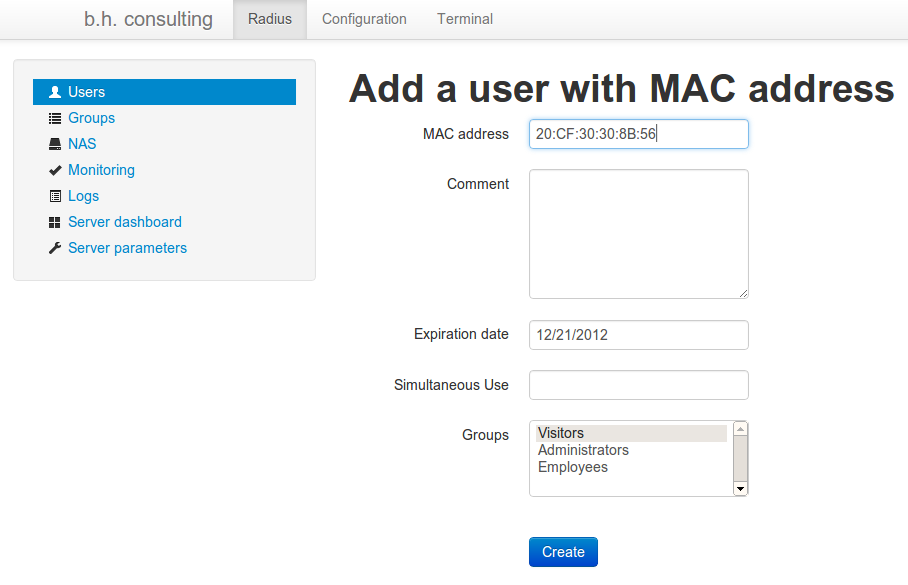
\includegraphics[width=\textwidth]{img/capture4.png}
\end{frame}

\part{Work organization}
\frame{\partpage}
\section{Work organization}

\begin{frame}{Team presentation}
    \begin{itemize}[<+->]
	\item {\bf Julien Guépin} - \emph{Software Engineering}
	\vfill
	\item {\bf Marc Pinhède} - \emph{Embedded Software}
	\vfill
	\item {\bf Julien Vaubourg} - \emph{Telecoms, Networks and Services}
	\vfill
	\item {\bf Nicolas Bouget} - \emph{Telecoms, Networks and Services}
    \end{itemize}
\end{frame}

\begin{frame}{VM Project}
    \begin{center}
    
\includegraphics[width=160pt]{img/vmproject_logo.png}
    \end{center}
    \begin{itemize}[<+->]
	\item Software used to \textbf{assist the team}
    	\vfill
    	\item Assist the project leader to \textbf{follow tasks progress}
    	\vfill
    	\item \textbf{Gantt chart} auto-generation
    	\vfill
    	\item \textbf{Meeting report} system
    \end{itemize}
\end{frame}

\begin{frame}{Planning}
%\begin{center}
	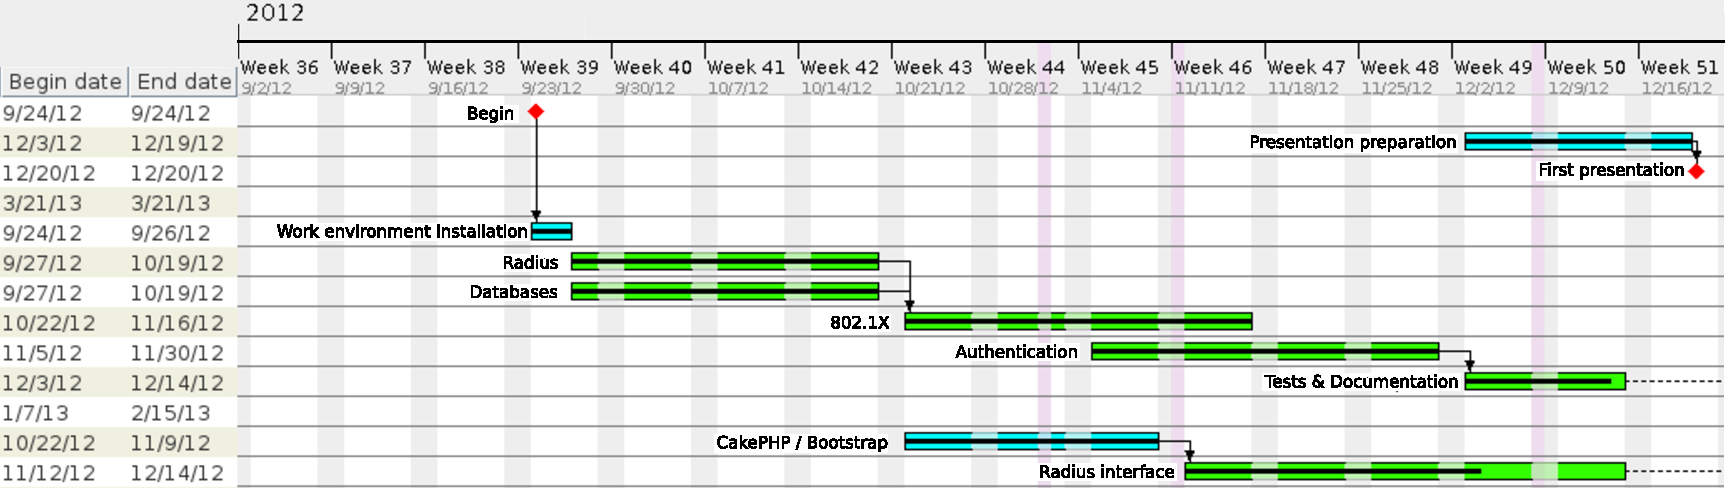
\includegraphics[width=330pt]{img/gantt_en_part1.pdf}\\
~\\
	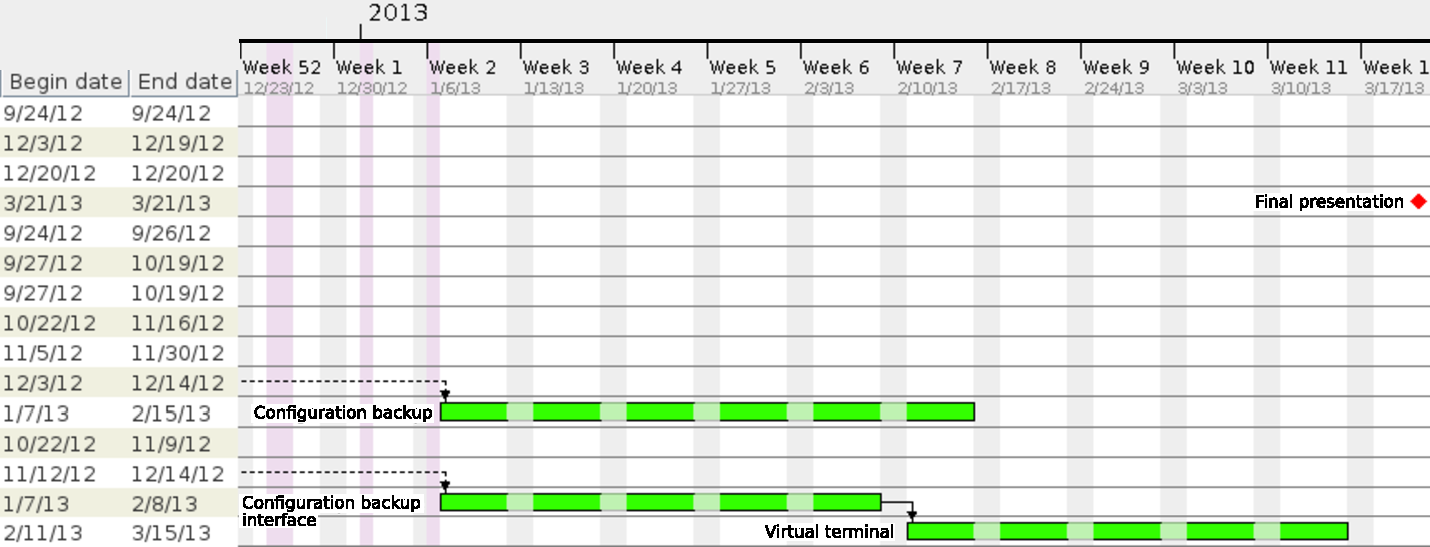
\includegraphics[height=70pt]{img/gantt_en_part2.pdf}
%\end{center}
\end{frame}

\begin{frame}{Meetings}
\begin{itemize}
    \item \textbf{Monthly} meeting (\textbf{Jean-François Scheid})
	\vspace{0.2cm}
	\begin{itemize}
	\item Project progression summary
	\item Report of any major problem
	\end{itemize}
	\vspace{0.8cm}\pause
    \item \textbf{Weekly} meeting (\textbf{Guillaume Roche})
	\vspace{0.2cm}
	\begin{itemize}
	\item Week summary
	\item Questions
	\item Directions
	\end{itemize}
    \end{itemize}
\end{frame}

\begin{frame}{Current progression}
    \begin{center}
         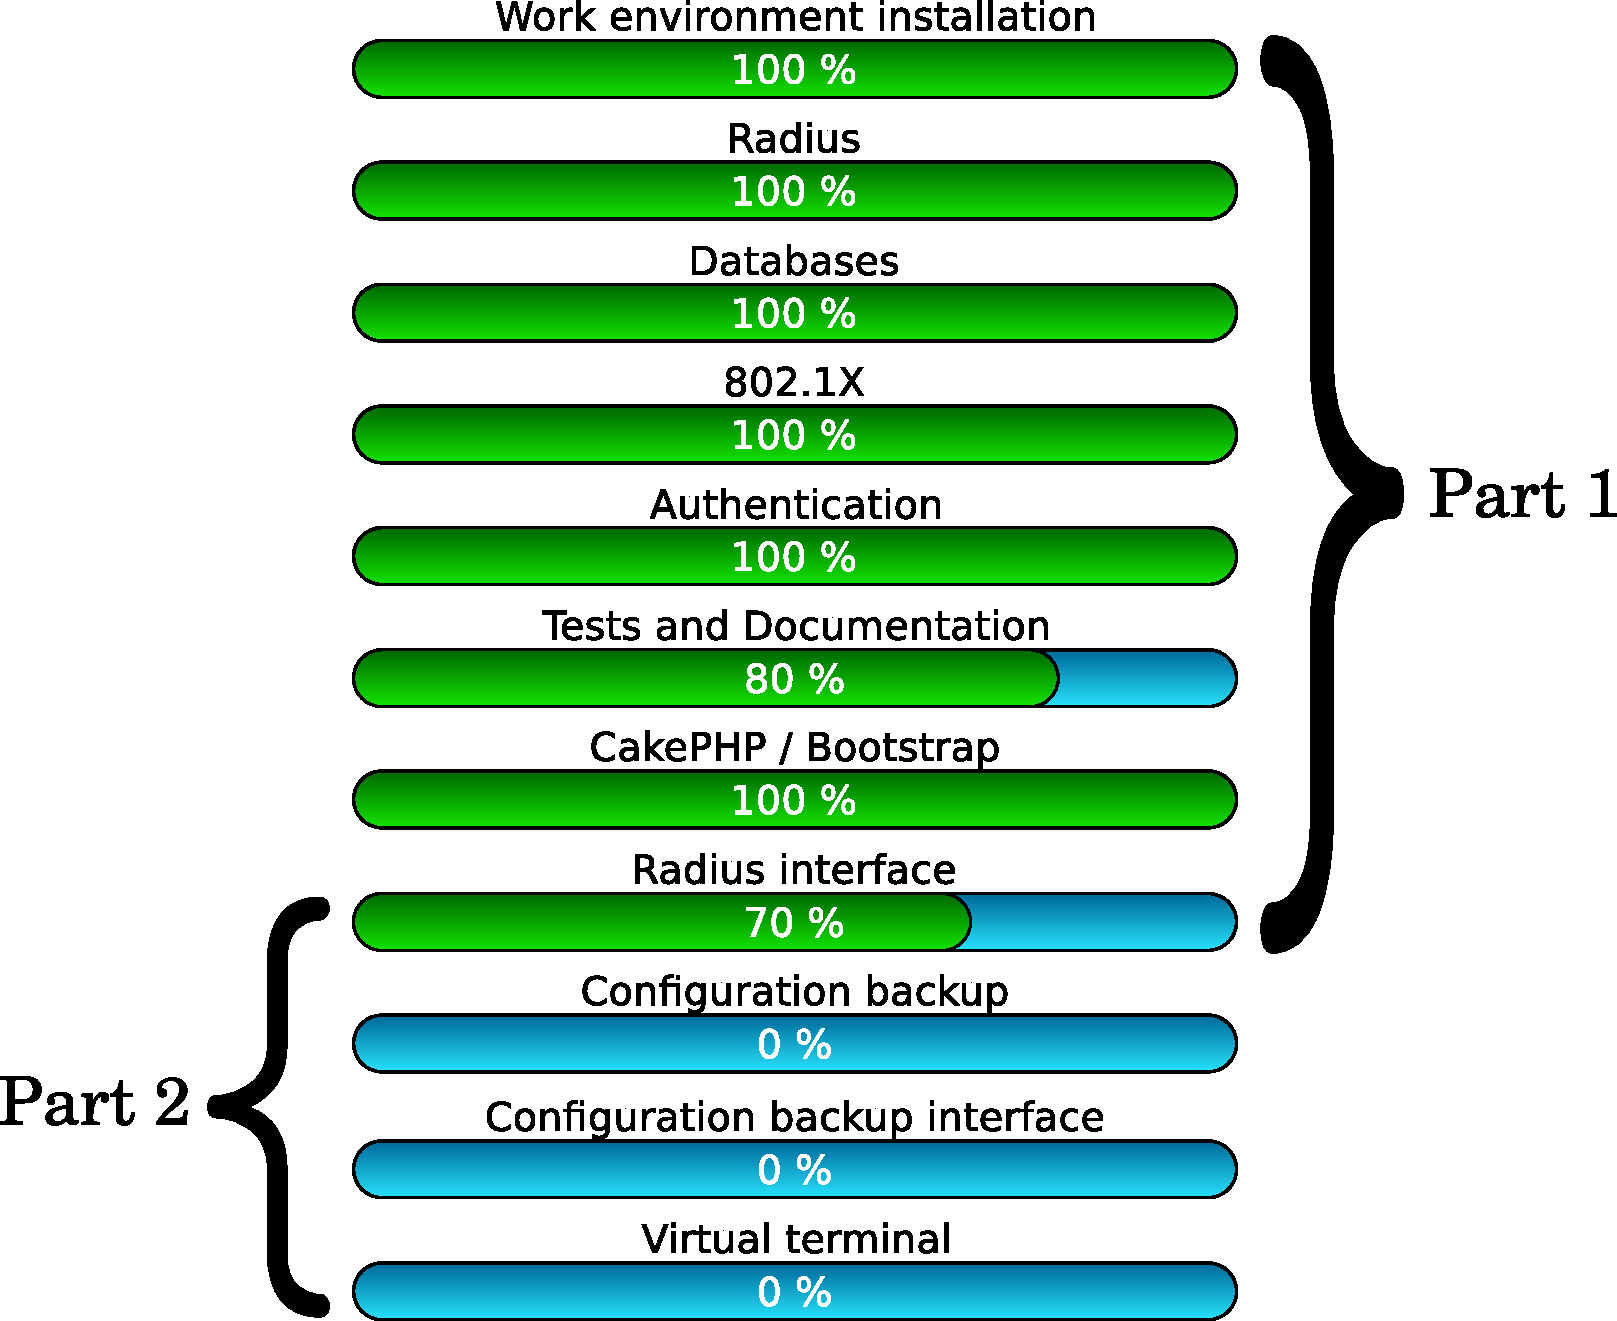
\includegraphics[width=200pt]{img/progress.pdf}
    \end{center}
\end{frame}

\begin{frame}{Conclusion}
    \begin{itemize}
	\item \textbf{First part almost finished}
	\vfill
	\item \textbf{Some difficulties} because of needed equipments
	\vfill
	\item \textbf{Good interest} of the team about the project
	\vfill
	\item \textbf{Quick reaction} from B.H. Consulting
    \end{itemize}
\end{frame}

\begin{frame}{}
    \begin{center}
	{\usebeamercolor[fg]{structure}\huge{Thank you for your attention!\\~\\~\\}}
	{\usebeamercolor[fg]{structure}\huge{Questions?}}
    \end{center}
\end{frame}

\end{document}
